\documentclass[10pt,twocolumn]{article}

\usepackage[T1]{fontenc}
\usepackage{lmodern}
\usepackage{microtype}
\usepackage{xspace}
\usepackage[letterpaper,top=0.67in,bottom=0.72in,left=0.68in,right=0.68in,columnsep=0.24in]{geometry}
\usepackage{amsmath}
\usepackage{booktabs}
\usepackage{graphicx}
\usepackage{tabularx}
\usepackage{xcolor}
\usepackage{tikz}
\usepackage{pgfplots}
\usepackage[font=small,labelfont=bf]{caption}
\usepackage[hidelinks]{hyperref}
\usepackage{url}

\pgfplotsset{compat=1.17}
\usepgfplotslibrary{colormaps}
\usetikzlibrary{arrows.meta,positioning,fit}
\setlength{\parindent}{1em}
\setlength{\parskip}{0pt}
\setlength{\textfloatsep}{7pt plus 2pt minus 2pt}
\setlength{\floatsep}{6pt plus 2pt minus 2pt}
\setlength{\intextsep}{6pt plus 2pt minus 2pt}
\setlength{\abovecaptionskip}{3pt}
\setlength{\belowcaptionskip}{0pt}
\renewcommand{\arraystretch}{1.08}

\definecolor{tidalblue}{HTML}{276FBF}
\definecolor{tidalcyan}{HTML}{38A3A5}
\definecolor{tidalorange}{HTML}{F08A4B}
\definecolor{tidalpurple}{HTML}{7C3AED}
\definecolor{tidalgray}{HTML}{F2F4F7}
\definecolor{tidaldark}{HTML}{25313C}

\newcommand{\system}{\textsc{Tidal}\xspace}
\newcommand{\res}{\textsc{res}\xspace}
\newcommand{\pool}{\textsc{Pool}\xspace}
\newcommand{\privatefour}{\textsc{private-v4}\xspace}
\newcommand{\capthree}{\textsc{pressure-cap3}\xspace}
\newcolumntype{Y}{>{\raggedright\arraybackslash}X}
\newcolumntype{P}[1]{>{\raggedright\arraybackslash}p{#1}}

\makeatletter
\renewcommand\section{\@startsection{section}{1}{\z@}%
  {-1.7ex plus -.4ex minus -.2ex}%
  {.7ex plus .2ex}%
  {\normalfont\large\bfseries}}
\renewcommand\subsection{\@startsection{subsection}{2}{\z@}%
  {-1.2ex plus -.3ex minus -.2ex}%
  {.45ex plus .15ex}%
  {\normalfont\normalsize\bfseries}}
\makeatother

\begin{document}
\hypersetup{
  pdftitle={Tidal: Direction-Paired Virtual-Channel Buffer Pooling with a 1R1W Shared Pool},
  pdfauthor={Changxun Pan and Liming Wang},
  pdfkeywords={on-chip networks, virtual channels, shared buffers, Garnet, gem5}
}

\twocolumn[
\begin{@twocolumnfalse}
\begin{center}
  {\LARGE\bfseries Tidal: Direction-Paired Virtual-Channel Buffer Pooling\\
  with a 1R1W Shared Pool\par}
  \vspace{0.55em}
  {\large Changxun Pan \qquad Liming Wang\par}
  \vspace{0.2em}
  {\small Equal contribution: 50\% each\par}
\end{center}
\vspace{-0.2em}
\begin{abstract}
Conventional on-chip routers bind virtual-channel (VC) storage to individual
input directions. This organization strands storage when one direction is
congested and its opposite peer is idle. \system reorganizes the same eight
VC slots per opposing-direction pair into two two-slot reserved regions and a
four-slot shared \pool. Each direction retains one private adaptive VC and one
private escape VC. The \pool provides only one read and one write service per
cycle; alternating read phases let one side inspect its reserved region while
the other inspects the \pool. Four conserved \pool credits control admission.
A pressure policy moves released credits toward the side with fuller reserved
storage, keeps the previous owner on ties, caps ownership at three, and
reclaims only idle peer-owned slots on demand.

We implement the design in gem5 Garnet and evaluate an equal-storage
four-private-VC baseline. Across 1,077 main-matrix simulations, all runs
completed without deadlock and recorded zero cross-direction \pool read
conflicts. Under persistent 90/10 X-direction skew with eight-cycle links,
\system lowers network latency by 9.2\% and extends the stable offered
rate from 0.08 to 0.10. At a fully skewed point beyond baseline saturation it
delivers 1.818 times as many packets. Under tornado traffic, pressure-aware
credit control lowers latency by 4.85\%, whereas blind round-robin ownership
loses 56.5\% throughput. Balanced, short-link, and rapidly reversing traffic
can be slower. The results identify persistent directional skew near an input
credit limit as the useful operating region and motivate timing and RTL cost
validation.
\end{abstract}
\vspace{0.55em}
\noindent\textbf{Keywords:} on-chip networks, virtual channels, shared buffers,
credit flow control, Garnet, gem5
\vspace{0.8em}
\end{@twocolumnfalse}
]

\section{Introduction}

Virtual-channel (VC) flow control improves throughput by multiplexing logical
channels over physical links, and it turns buffer organization into a central
router design choice: input buffers account for a large share of an on-chip
router's area and power budget~\cite{dally1992virtual,nicopoulos2006vichar}.
Garnet models a pipelined, credit-controlled network inside gem5 and is widely
used to study these tradeoffs~\cite{agarwal2009garnet,binkert2011gem5}. Its
conventional organization is fully private: every input direction owns a
fixed set of VCs, and storage never migrates.

Private storage is wasteful precisely when the network is most stressed.
Directionally skewed traffic---tornado permutations, biased
dimension-ordered flows---drives one member of an opposing-direction pair
against its input-credit limit while the peer sits nearly empty. The cost is
measurable: at eight-cycle link latency, a fully skewed workload saturates a
private four-VC baseline at an offered rate of 0.08, whereas the same eight
buffer slots per pair, reorganized by \system, sustain 0.10 and deliver
1.818 times as many packets beyond the baseline's saturation point
(Section~\ref{sec:eval-skew}).

Elastic buffers are the classic remedy, but prior schemes buy their
elasticity with multiported storage or wide arbitration, and industrial
credit pools share only among the message classes of one link
(Section~\ref{sec:background}). Our question is narrower: \emph{can an
equal-capacity, direction-paired buffer recover useful elasticity while
exposing only one shared read and one shared write service per pair and
cycle?}

This paper makes four contributions:
\begin{itemize}
  \setlength{\itemsep}{0pt}
  \setlength{\topsep}{2pt}
  \item an equal-storage organization with three independent pairs per router,
  one private adaptive VC and one escape VC per direction, and four movable
  adaptive slots per pair;
  \item an alternating read schedule and a one-write admission guard that
  implement the shared bank as 1R1W;
  \item a conserved ownership-credit policy combining pressure, sticky ties,
  a three-credit cap, and idle-slot reclaim; and
  \item a 1,077-run evaluation that reports both the favorable region and
  the workloads where the fixed phase schedule is counterproductive.
\end{itemize}

\section{Background and Motivation}
\label{sec:background}

A conventional four-VC input assigns four physical VC slots to each
direction. Credit round-trip time determines how quickly a released downstream
slot can be reused. With one-flit control traffic and an approximately
17-cycle credit loop at link latency $L=8$, four slots impose an idealized
zero-contention input-credit bound of
\begin{equation}
  \lambda_{\mathrm{credit}} \approx \frac{4}{17}=0.235
  \quad\text{flits/cycle}.
\end{equation}
The exact saturation point can be lower because routing, output contention,
and switch arbitration intervene. This bound is \emph{per direction}, and
that is the problem: under persistent $+X$ skew the E input exhausts its
credits and stalls its upstream sender while the four W slots one crossbar
port away stay idle. The router holds enough total storage for the offered
load; it is partitioned along a boundary the traffic does not respect.

Elastic buffers are the classic remedy. DAMQ buffers manage one physical
buffer as linked lists whose queues grow with demand~\cite{tamir1992damq};
ViChaR dispenses VCs themselves from a unified
buffer~\cite{nicopoulos2006vichar}; ElastiStore backs all VCs of a port with
a shared slack buffer~\cite{seitanidis2014elastistore}. All share storage
\emph{within} one input port, and all pay in multiported storage, per-flit
pointer management, or wider arbitration---costs that grow with the number of
sharers. Production interconnects settled on a more conservative contract:
a small private reservation per traffic class plus one shared, credit-managed
pool (QPI/UPI's VN0/VNA~\cite{intel2009qpi}, Omni-Path's dedicated and
shared receive regions~\cite{birrittella2015omnipath}, and CMN-700's
per-link pools~\cite{arm2021cmn700}). But these pools share among the
message classes of one physical link, so directional skew strands storage
exactly as in the private baseline.

\system combines the two: it applies the reserved-plus-pooled contract
\emph{across} a router's two opposing inports---the axis skewed traffic
actually unbalances---while constraining the shared bank up front to one read
and one write per cycle, a budget conventional SRAM provides. Pairing
exactly two sharers keeps the sharing hardware small, and admission moves by
conserved ownership credits rather than per-flit pointers. Deadlock safety
stays outside the elastic domain: every direction keeps a private
deterministic escape VC, consistent with separating deadlock avoidance from
adaptive resource use~\cite{dally1987deadlock,duato1993theory}.

\section{Architecture}

\subsection{Direction-paired storage}

Each router instantiates East/West, North/South, and Up/Down pairs. Figure~\ref{fig:pair}
shows one pair. For each direction, \res contains one private adaptive VC and
one private escape VC. The pair shares four adaptive slots:
\begin{equation}
  2(1_{\mathrm{private}}+1_{\mathrm{escape}})
  +4_{\mathrm{pool}}=8\ \mathrm{slots}.
\end{equation}
This equals the eight slots in two four-VC private inputs, so performance
comparisons preserve total storage.

\begin{figure}[t]
\centering
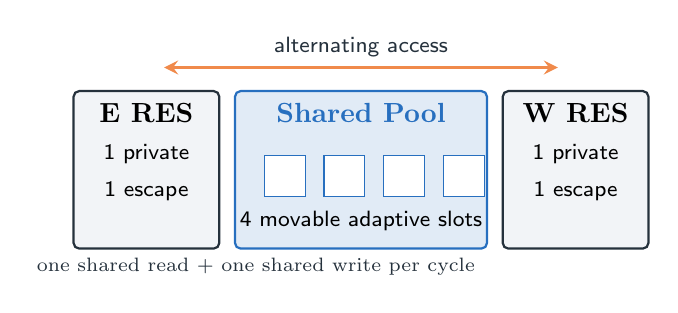
\begin{tikzpicture}[font=\sffamily\footnotesize,>=stealth]
  \draw[rounded corners=2pt,fill=tidalgray,draw=tidaldark,thick]
    (0,0) rectangle (1.85,2.0);
  \draw[rounded corners=2pt,fill=tidalblue!14,draw=tidalblue,thick]
    (2.05,0) rectangle (5.25,2.0);
  \draw[rounded corners=2pt,fill=tidalgray,draw=tidaldark,thick]
    (5.45,0) rectangle (7.30,2.0);
  \node[font=\bfseries] at (0.925,1.72) {E RES};
  \node at (0.925,1.20) {1 private};
  \node at (0.925,0.72) {1 escape};
  \node[font=\bfseries,text=tidalblue] at (3.65,1.72) {Shared Pool};
  \foreach \x in {2.42,3.18,3.94,4.70}
    \draw[fill=white,draw=tidalblue] (\x,0.66) rectangle ++(0.52,0.52);
  \node at (3.65,0.35) {4 movable adaptive slots};
  \node[font=\bfseries] at (6.375,1.72) {W RES};
  \node at (6.375,1.20) {1 private};
  \node at (6.375,0.72) {1 escape};
  \draw[<->,very thick,tidalorange] (1.15,2.30) -- node[above,text=tidaldark]
    {alternating access} (6.15,2.30);
  \node[anchor=east,font=\scriptsize,text=tidaldark] at (5.22,-0.23)
    {one shared read + one shared write per cycle};
\end{tikzpicture}
\caption{One direction pair. Every router contains three copies: E/W, N/S,
and U/D. Capacity matches the private four-VC baseline.}
\label{fig:pair}
\end{figure}

\pool membership follows \emph{true ingress}, not the selected output. A flit
entering from X may occupy the X-pair \pool and later depart through Y or Z.
Each pooled flit stores its ingress direction and upstream VC so that its
credit returns to the correct sender.

\subsection{Router-level on-chip organization}

Figure~\ref{fig:router-microarch} places one pair inside a router tile. The
same structure is replicated for E/W, N/S, and U/D. The two incoming links
retain independent \res banks. Their adaptive arrivals also feed one shared
\pool write arbiter. Section~\ref{sec:physical} details the pair's internal
construction.

\begin{figure*}[t]
\centering
\resizebox{\textwidth}{!}{%
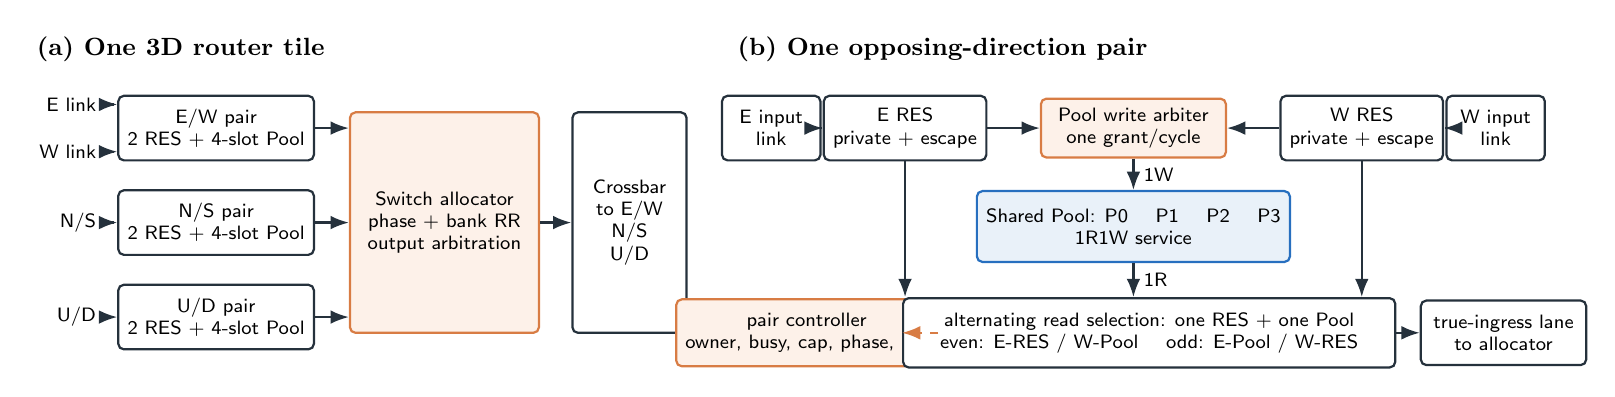
\begin{tikzpicture}[
  font=\sffamily\scriptsize,
  >=Latex,
  box/.style={draw=tidaldark,rounded corners=2pt,thick,fill=white,
    align=center,minimum height=0.82cm},
  ctrl/.style={draw=tidalorange!90!black,rounded corners=2pt,thick,
    fill=tidalorange!12,align=center},
  poolbox/.style={draw=tidalblue,rounded corners=2pt,thick,
    fill=tidalblue!10,align=center},
  flow/.style={->,thick,draw=tidaldark},
  cflow/.style={->,thick,dashed,draw=tidalorange!90!black}
]
  % Panel (a): router tile
  \node[font=\bfseries\small,anchor=west] at (0,4.25) {(a) One 3D router tile};
  \node[box,minimum width=2.2cm] (ew) at (2.40,3.25)
    {E/W pair\\2 RES + 4-slot Pool};
  \node[box,minimum width=2.2cm] (ns) at (2.40,2.05)
    {N/S pair\\2 RES + 4-slot Pool};
  \node[box,minimum width=2.2cm] (ud) at (2.40,0.85)
    {U/D pair\\2 RES + 4-slot Pool};
  \node[ctrl,minimum width=2.4cm,minimum height=2.8cm] (sa) at (5.30,2.05)
    {Switch allocator\\phase + bank RR\\output arbitration};
  \node[box,minimum width=1.45cm,minimum height=2.8cm] (xbar) at (7.65,2.05)
    {Crossbar\\to E/W\\N/S\\U/D};
  \draw[flow] (ew.east) -- (sa.west |- ew.east);
  \draw[flow] (ns.east) -- (sa.west |- ns.east);
  \draw[flow] (ud.east) -- (sa.west |- ud.east);
  \draw[flow] (sa) -- (xbar);
  \node[anchor=east] at (1.00,3.55) {E link};
  \node[anchor=east] at (1.00,2.95) {W link};
  \node[anchor=east] at (1.00,2.05) {N/S};
  \node[anchor=east] at (1.00,0.85) {U/D};
  \draw[flow] (1.10,3.55) -- (ew.west |- 2.40,3.55);
  \draw[flow] (1.10,2.95) -- (ew.west |- 2.40,2.95);
  \draw[flow] (1.10,2.05) -- (ns.west);
  \draw[flow] (1.10,0.85) -- (ud.west);

  % Panel (b): pair datapath
  \node[font=\bfseries\small,anchor=west] at (8.90,4.25)
    {(b) One opposing-direction pair};
  \node[box,minimum width=1.25cm] (elin) at (9.45,3.25) {E input\\link};
  \node[box,minimum width=1.25cm] (wlin) at (18.65,3.25) {W input\\link};
  \node[box,minimum width=1.85cm] (eres) at (11.15,3.25)
    {E RES\\private + escape};
  \node[box,minimum width=1.85cm] (wres) at (16.95,3.25)
    {W RES\\private + escape};
  \node[ctrl,minimum width=2.35cm] (warb) at (14.05,3.25)
    {Pool write arbiter\\one grant/cycle};
  \node[poolbox,minimum width=3.95cm,minimum height=0.90cm] (pool) at (14.05,2.00)
    {Shared Pool: P0 \quad P1 \quad P2 \quad P3\\1R1W service};
  \node[ctrl,minimum width=2.35cm,minimum height=0.85cm] (state) at (9.90,0.65)
    {pair controller\\owner, busy, cap, phase, RR};
  \node[box,minimum width=6.25cm,minimum height=0.88cm] (rmux) at (14.25,0.65)
    {alternating read selection: one RES + one Pool\\even: E-RES / W-Pool \quad odd: E-Pool / W-RES};
  \node[box,minimum width=2.10cm] (lane) at (18.75,0.65)
    {true-ingress lane\\to allocator};

  \draw[flow] (elin) -- (eres);
  \draw[flow] (wlin) -- (wres);
  \draw[flow] (eres) -- (warb);
  \draw[flow] (wres) -- (warb);
  \draw[flow] (warb) -- node[right]{1W} (pool);
  \draw[flow] (eres.south) -- (eres.south |- rmux.north);
  \draw[flow] (pool.south) -- node[right]{1R} (pool.south |- rmux.north);
  \draw[flow] (wres.south) -- (wres.south |- rmux.north);
  \draw[flow] (rmux) -- (lane);
  \draw[cflow] (state) -- (rmux);
\end{tikzpicture}
}
\caption{Proposed on-chip organization. (a) Three direction-pair controllers
operate in parallel around the normal Garnet switch allocator and crossbar.
(b) One pair exposes a single shared Pool read and write service. RES access
remains separate; solid arrows are flit/request paths and the sole dashed
arrow is controller state. The Pool result is placed on the flit's
true-ingress lane.}
\label{fig:router-microarch}
\end{figure*}

\subsection{One-read, one-write service}

The \pool accepts at most one read and one write service per pair, control
virtual network, and cycle. Read phases are complementary:
\begin{center}
\small
\begin{tabular}{lll}
\toprule
Phase & Side 0 (E/N/U) & Side 1 (W/S/D)\\
\midrule
Even & \res & \pool\\
Odd  & \pool & \res\\
\bottomrule
\end{tabular}
\end{center}
Thus E can inspect \res while W inspects the \pool, and the roles reverse next
cycle. Cycle parity structurally eliminates simultaneous cross-direction
\pool reads. Ordinary VC and switch arbitration still select among eligible
flits inside the active bank.

A per-pair write guard permits one adaptive \pool allocation each cycle. If
both sides arrive, the second arrival may still use its private adaptive VC
when that reserved credit is available; otherwise it waits. Escape storage
never enters the shared bank and follows deterministic non-wrapping XYZ
routing.

The port count must be stated precisely. A pair can perform two useful reads
in a cycle: one from the selected side's \res and one from the shared \pool.
Only the latter consumes the Pool's single read port. A \res write is likewise
independent of the Pool write. For the present one-flit control traffic, Pool
VC allocation and data arrival are one-to-one, so accepting at most one new
Pool allocation per pair and cycle models a single Pool write service. A
multi-flit extension would need a separate per-flit write schedule.

\subsection{Physical construction of one pair}
\label{sec:physical}

Figure~\ref{fig:bank} draws the blocks that the service contract above
implies for one pair and control vnet.

\begin{figure}[t]
\centering
\resizebox{\columnwidth}{!}{%
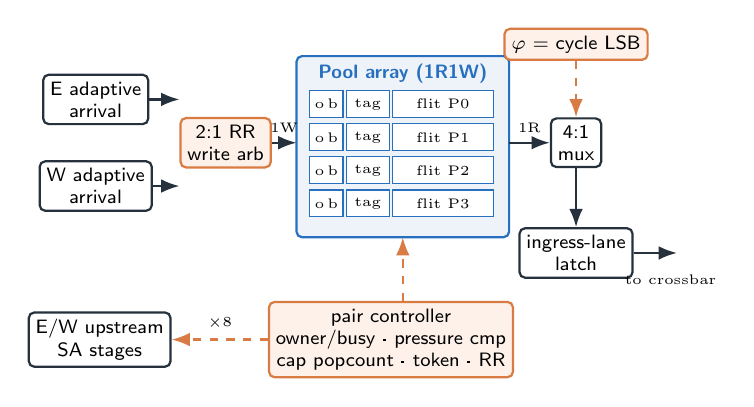
\begin{tikzpicture}[font=\sffamily\scriptsize,>=Latex,
  blk/.style={draw=tidaldark,thick,rounded corners=2pt,fill=white,
    align=center,inner sep=2.5pt},
  ctl/.style={draw=tidalorange!90!black,thick,rounded corners=2pt,
    fill=tidalorange!12,align=center,inner sep=2.5pt},
  arr/.style={->,thick,draw=tidaldark},
  sbd/.style={->,thick,dashed,draw=tidalorange!90!black}]

  \node[blk] (ereq) at (0.85,4.05) {E adaptive\\arrival};
  \node[blk] (wreq) at (0.85,2.95) {W adaptive\\arrival};
  \node[ctl] (warb) at (2.5,3.5) {2:1 RR\\write arb};
  \draw[arr] (ereq.east) -- (warb.west |- ereq.east);
  \draw[arr] (wreq.east) -- (warb.west |- wreq.east);

  \draw[draw=tidalblue,thick,rounded corners=2pt,fill=tidalblue!8]
    (3.4,2.3) rectangle (6.1,4.6);
  \node[font=\sffamily\bfseries\scriptsize,text=tidalblue]
    at (4.75,4.38) {Pool array (1R1W)};
  \foreach \i/\y in {0/3.82,1/3.40,2/2.98,3/2.56} {
    \draw[fill=white,draw=tidalblue] (3.57,\y) rectangle ++(0.42,0.34);
    \draw[fill=white,draw=tidalblue] (4.03,\y) rectangle ++(0.55,0.34);
    \draw[fill=white,draw=tidalblue] (4.62,\y) rectangle ++(1.28,0.34);
    \node[font=\tiny] at (3.78,\y+0.17) {o\,b};
    \node[font=\tiny] at (4.305,\y+0.17) {tag};
    \node[font=\tiny] at (5.26,\y+0.17) {flit P\i};
  }
  \draw[arr] (warb.east) -- node[above,font=\tiny]{1W} (3.4,3.5);

  \node[blk] (rmux) at (6.95,3.5) {4:1\\mux};
  \draw[arr] (6.1,3.5) -- node[above,font=\tiny]{1R} (rmux.west);
  \node[blk] (lane) at (6.95,2.1) {ingress-lane\\latch};
  \draw[arr] (rmux.south) -- (lane.north);
  \draw[arr] (lane.east) -- ++(0.55,0);
  \node[font=\tiny,anchor=north] at (8.15,1.95) {to crossbar};

  \node[ctl] (phase) at (6.95,4.75) {$\varphi$ = cycle LSB};
  \draw[sbd] (phase.south) -- (rmux.north);

  \node[ctl] (pc) at (4.6,1.0)
    {pair controller\\owner/busy · pressure cmp\\cap popcount · token · RR};
  \draw[sbd] (4.75,0 |- pc.north) -- (4.75,2.3);
  \node[blk] (esa) at (0.9,1.0) {E/W upstream\\SA stages};
  \draw[sbd] (pc.west) -- node[above,font=\tiny]{$\times$8} (esa.east);
\end{tikzpicture}%
}
\caption{Construction of one pair's shared bank: a two-request arbiter in
front of the single write port, a phase-gated 4:1 read multiplexer onto the
winner's true-ingress crossbar lane, and a local pair controller whose
owner/busy bits both upstream allocators observe over a narrow sideband.
o, b = per-slot owner and busy bits.}
\label{fig:bank}
\end{figure}

\textbf{Storage.} The four \pool entries are flit-wide registers with a
sidecar tag, built either as one central four-entry 1R1W register-file macro
or as two two-entry halves colocated with each side's \res bank and numbered
globally; the Garnet model mirrors the second layout
(Section~\ref{sec:vc-map}). Each entry holds the 128-bit flit of the default
Garnet link plus a seven-bit tag---true-ingress side (1 bit), credit inport
(3 bits), and upstream logical VC (3 bits). The tag exists only because a
slot may be borrowed by the opposite side; \res entries need none.

\textbf{Read path.} The phase bit $\varphi$ is the low bit of the router
cycle counter. Per side it masks which bank's requests enter switch
allocation; within the active \pool bank a masked round-robin pointer picks
one eligible entry, and a 4:1 flit multiplexer steers it onto the winner's
true-ingress lane. The crossbar keeps one port per direction and gains none.

\textbf{Write path.} Adaptive arrivals of both sides meet a two-request
round-robin arbiter in front of the single write port; a token flop cleared
every cycle enforces the single grant. The loser falls back to its private
VC when that credit is free and otherwise waits upstream. \res writes bypass
the arbiter.

\textbf{Control state and policy logic.} Table~\ref{tab:state} counts the
pair controller's state: 18 control bits plus four seven-bit tags per pair
and vnet, under 5\% of the pair's 1{,}024 data bits. Pressure is a
combinational count of each side's active \res VCs (range 0--2), so a
release grant is a 2-bit compare; the cap check is a popcount of the four
owner bits against three. All policy logic is local to the downstream pair
controller.

\begin{table}[t]
\centering
\caption{Per-pair, per-vnet control state.}
\label{tab:state}
\small
\setlength{\tabcolsep}{4.5pt}
\begin{tabular}{lrl}
\toprule
State & Bits & Role\\
\midrule
owner$[0..3]$ & 4 & authorized side per slot\\
busy$[0..3]$ & 4 & in-flight guard (from VC-valid)\\
write token & 1 & one \pool write per cycle\\
bank RR pointers & 8 & read selection per side/bank\\
policy RR bit & 1 & write-arbiter fairness\\
ingress tags & $4\times7$ & credit return for borrowed slots\\
\midrule
total & 46 & $<5\%$ of 1{,}024 data bits\\
\bottomrule
\end{tabular}
\end{table}

\textbf{Ownership observation.} Owner and busy bits live at the downstream
controller, but the claim decision runs in the upstream allocator, which
therefore observes eight bits per pair and vnet over a one-way sideband (or
an upstream-mirrored copy updated by the same events). The simulator treats
this observation as combinational; Section~\ref{sec:timing} prices
registering it.

\textbf{Pipeline placement.} Upstream, the owner/busy check and the slot
claim run inside output-VC selection at switch allocation and consume the
write token in the claim cycle. Downstream, the phase mask gates input
arbitration, switch traversal is unchanged, and the release-time pressure
grant runs at tail departure together with the ordinary credit enqueue. The
event-level Garnet model does not synthesize these blocks; it enforces their
service limits and measures their utilization.

\section{Pool-Credit Control}

Each of the four shared slots has exactly one logical owner. For the E/W pair,
ownership obeys
\begin{equation}
  C_E+C_W=4,\qquad 1\leq C_E,C_W\leq 3.
\end{equation}
An owned \pool credit authorizes the corresponding upstream direction to
reserve an idle slot. Private and escape credits remain pinned.

\subsection{Two credit planes}

The implementation deliberately separates \emph{buffer occupancy} from
\emph{Pool ownership}. They are both called credits informally, but they have
different destinations and correctness roles:
\begin{table}[t]
\centering
\caption{The two credit planes in \system.}
\label{tab:credit-planes}
\small
\begin{tabularx}{\columnwidth}{@{}P{0.20\columnwidth}YY@{}}
\toprule
Plane & State and path & Meaning\\
\midrule
Occupancy &
Garnet OutputUnit VC state; returned on the real CreditLink to the upstream
port that sent the flit &
The physical slot is free; prevents overflow\\
Ownership &
One owner bit per Pool slot; selected by the downstream pair controller and
observed by either opposing sender &
This direction may allocate the idle slot\\
\bottomrule
\end{tabularx}
\end{table}

Returning an occupancy credit never changes its physical path. Even when an E
flit was placed in the W-hosted half of the \pool, stored metadata identifies
the true E ingress link and the original upstream logical VC. The ordinary
free credit is sent back on E's CreditLink. Independently, the downstream
owner bit may stay with E or move to W. A sender whose logical VC has become
idle must still pass the owner-table check before reusing that Pool slot.

\subsection{Allocation, release, and handoff}

Figure~\ref{fig:credit-life} follows one one-flit packet. The upstream router
first searches its private adaptive VC, then idle Pool slots it already owns,
then idle peer-owned slots that it may reclaim under the cap. A successful
Pool choice atomically sets \texttt{owner[slot]}, sets
\texttt{busy[slot]}, and consumes the pair's write token for that cycle. The
logical Pool VC ID travels with the flit. At the downstream router, that ID is
mapped to one of four physical Pool entries and tagged with true ingress,
credit input port, and upstream VC ID.

\begin{figure*}[t]
\centering
\resizebox{\textwidth}{!}{%
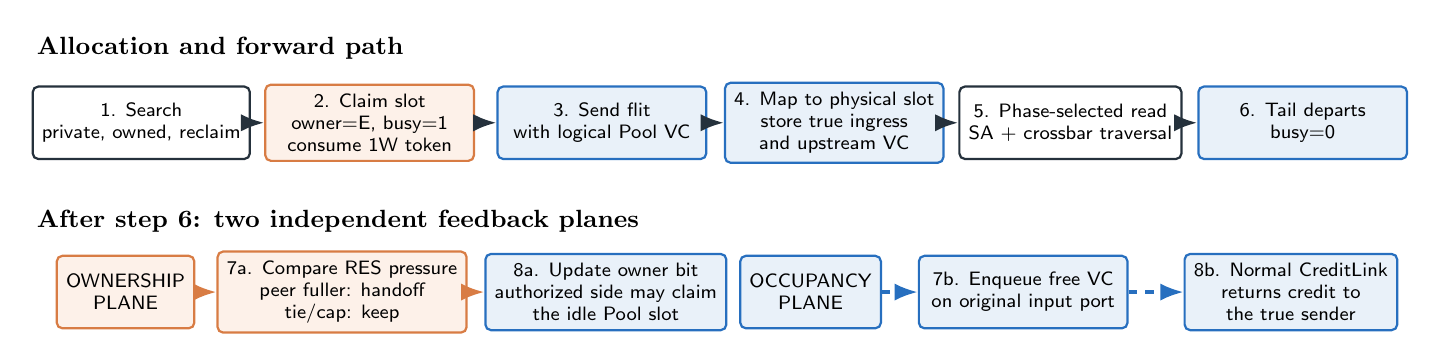
\begin{tikzpicture}[
  font=\sffamily\scriptsize,
  >=Latex,
  stagebox/.style={draw=tidaldark,rounded corners=2pt,thick,fill=white,
    align=center,minimum width=2.55cm,minimum height=0.92cm},
  event/.style={draw=tidalblue,rounded corners=2pt,thick,fill=tidalblue!10,
    align=center,minimum width=2.65cm,minimum height=0.92cm},
  decision/.style={draw=tidalorange!90!black,rounded corners=2pt,thick,
    fill=tidalorange!12,align=center,minimum width=2.65cm,minimum height=0.92cm},
  flow/.style={->,very thick,draw=tidaldark},
  ownership/.style={->,very thick,dashed,draw=tidalorange!90!black},
  occupancy/.style={->,very thick,dashed,draw=tidalblue}
]
  \node[font=\bfseries\small,anchor=west] at (0,2.85)
    {Allocation and forward path};
  \node[stagebox] (search) at (1.45,1.90)
    {1. Search\\private, owned, reclaim};
  \node[decision] (claim) at (4.35,1.90)
    {2. Claim slot\\owner=E, busy=1\\consume 1W token};
  \node[event] (send) at (7.30,1.90)
    {3. Send flit\\with logical Pool VC};
  \node[event] (map) at (10.25,1.90)
    {4. Map to physical slot\\store true ingress\\and upstream VC};
  \node[stagebox] (serve) at (13.25,1.90)
    {5. Phase-selected read\\SA + crossbar traversal};
  \node[event] (free) at (16.20,1.90)
    {6. Tail departs\\busy=0};
  \draw[flow] (search) -- (claim);
  \draw[flow] (claim) -- (send);
  \draw[flow] (send) -- (map);
  \draw[flow] (map) -- (serve);
  \draw[flow] (serve) -- (free);

  \node[font=\bfseries\small,anchor=west] at (0,0.65)
    {After step 6: two independent feedback planes};

  \node[decision,minimum width=1.65cm] (ownerlane) at (1.25,-0.25)
    {OWNERSHIP\\PLANE};
  \node[decision] (pressure) at (4.00,-0.25)
    {7a. Compare RES pressure\\peer fuller: handoff\\tie/cap: keep};
  \node[event] (ownergrant) at (7.35,-0.25)
    {8a. Update owner bit\\authorized side may claim\\the idle Pool slot};
  \draw[ownership] (ownerlane) -- (pressure);
  \draw[ownership] (pressure) -- (ownergrant);

  \node[event,minimum width=1.65cm] (occlane) at (9.95,-0.25)
    {OCCUPANCY\\PLANE};
  \node[event] (enqueuecredit) at (12.65,-0.25)
    {7b. Enqueue free VC\\on original input port};
  \node[event] (returncredit) at (16.05,-0.25)
    {8b. Normal CreditLink\\returns credit to\\the true sender};
  \draw[occupancy] (occlane) -- (enqueuecredit);
  \draw[occupancy] (enqueuecredit) -- (returncredit);
\end{tikzpicture}
}
\caption{Pool-credit lifecycle. The ordinary free credit returns to the actual
sender, whereas the released slot's ownership may be granted to either side.
The two non-crossing feedback lanes are both triggered by step 6. The
simulator models the owner-table change with no additional grant delay.}
\label{fig:credit-life}
\end{figure*}

When the tail wins switch traversal, the downstream router first clears the
busy bit and then evaluates the release policy. Table~\ref{tab:credit-rules}
gives the exact state transitions for the proposed pressure policy.

\begin{table*}[t]
\centering
\caption{Exact allocation and return rules for direction $d$ and peer
$\bar d$. An owner change is legal only for an idle slot.}
\label{tab:credit-rules}
\small
\begin{tabularx}{\textwidth}{@{}P{0.15\textwidth}P{0.29\textwidth}P{0.31\textwidth}Y@{}}
\toprule
Event & Guard / priority & Atomic state update & Result\\
\midrule
Private allocation &
Private adaptive VC is idle &
Reserve the private VC; Pool state unchanged &
No Pool port consumed\\
Owned Pool allocation &
Private busy; Pool 1W token free; an idle slot has
\(\mathrm{owner}[s]=d\) &
\(\mathrm{busy}[s]\leftarrow1\); record current-cycle write token &
Send using logical VC \(1+s\)\\
Demand reclaim &
No usable owned slot; 1W token free; peer-owned \(s\) is idle;
\(C_d<\mathrm{cap}\) &
\(\mathrm{owner}[s]\leftarrow d\);
\(\mathrm{busy}[s]\leftarrow1\); consume write token &
Immediate reclaim; busy slots are never revoked\\
Second Pool request &
Current-cycle write token already consumed &
Do not allocate Pool; use private/escape only if independently legal &
Otherwise request waits\\
Pool tail release &
Selected Pool flit completes switch traversal &
\(\mathrm{busy}[s]\leftarrow0\); count RES occupancy on both sides &
Evaluate pressure below\\
Pressure handoff &
\(\mathrm{RESused}_{\bar d}>\mathrm{RESused}_d\) and
\(C_{\bar d}<\mathrm{cap}\) &
\(\mathrm{owner}[s]\leftarrow\bar d\) &
Peer gains ownership; old sender still receives the normal free credit\\
Sticky keep &
Tie, own side fuller, or peer at cap &
\(\mathrm{owner}[s]\leftarrow d\) &
Preserve burst locality and the one-credit peer floor\\
\bottomrule
\end{tabularx}
\end{table*}

\textbf{Pressure grant.} When a pooled flit departs, its released credit is
assigned to the side whose \res occupancy is larger. This local pressure
signal approximates near-term need without adding a traffic predictor.

\textbf{Sticky tie.} Equal pressure preserves the previous owner. Stickiness
avoids credit oscillation and favors the side likely to continue a burst.

\textbf{Owner cap.} A cap of three lets a hot side borrow one additional slot
while guaranteeing one shared credit to its peer. Cap four is evaluated only
as a full-elasticity upper bound.

\textbf{On-demand reclaim.} Release-only movement can freeze if an idle owner
has no flit to release. A requester below its cap can therefore take an
\emph{idle} peer-owned slot immediately. Busy slots are never revoked. In the
current simulator, this owner-table update adds no cycle; Section~\ref{sec:limits}
treats this as an optimistic timing assumption.

The pressure value in the current code is the number of active private
adaptive and escape VCs in \res. The just-released Pool slot is excluded.
On equal pressure the old owner keeps the slot. If the preferred peer already
owns three slots, the cap overrides pressure and the old owner keeps it.

\subsection{Timing interpretation}
\label{sec:timing}

The ordinary occupancy credit is not idealized: it is inserted into the
original InputUnit's credit queue and scheduled on Garnet's CreditLink one
router cycle later. Ownership handoff is the optimistic component. The
simulator stores \texttt{owner[router][pair][vnet][slot]} at network scope, so
the newly authorized upstream direction observes the new owner without a
modeled sideband-wire or grant-register delay. A physical design needs a
one-way owner-grant signal from the downstream pair controller to both
opposing upstream allocators. Adding a registered one-cycle grant, or a
parameterized delay, is necessary before drawing frequency-sensitive
conclusions.

Blind owner round-robin is a useful control policy, but it is distinct from
the round-robin arbitration inside the read scheduler. Rotating ownership
without observing demand may park capacity at an inactive side.

\section{Garnet Implementation}

We implemented \system in gem5 Garnet's router, input unit, VC allocator, and
switch-allocation paths. The exact strict-1R1W snapshot is retained at
\path{1R1W/overlay}; its provenance records implementation commit
\path{dc43a290} and base commit \path{2eb6a4e}. Major additions are:
\begin{itemize}
  \setlength{\itemsep}{0pt}
  \setlength{\topsep}{2pt}
  \item physical-to-logical mapping for pair-global \pool slots;
  \item true-ingress and upstream-VC metadata for routing and credit return;
  \item complementary \res/\pool eligibility in switch allocation;
  \item a one-write-per-pair guard in downstream allocation;
  \item owner tables, pressure grants, cap enforcement, sticky ties, and
  idle-slot reclaim; and
  \item structural counters and X-biased/reversal synthetic traffic.
\end{itemize}

\subsection{Physical and logical VC mapping}
\label{sec:vc-map}

Each physical InputUnit still contains four control-vnet VC records. Offsets
0 and 3 are private; offsets 1 and 2 are that InputUnit's physical half of the
pair Pool. An internal link exposes six \emph{logical} IDs so either opposing
sender can name all four shared slots:
\begin{table}[t]
\centering
\caption{VC numbering for the four-physical-VC design.}
\label{tab:vc-map}
\small
\begin{tabular}{lll}
\toprule
Namespace & Offset(s) & Role\\
\midrule
Physical InputUnit & 0 & private adaptive\\
Physical InputUnit & 1, 2 & resident Pool half\\
Physical InputUnit & 3 & private escape\\
\midrule
Internal-link logical & 0 & private adaptive\\
Internal-link logical & 1--4 & pair-global Pool slots\\
Internal-link logical & 5 & private escape\\
\bottomrule
\end{tabular}
\end{table}

On arrival, \texttt{dpPhysMapLogicalVC} translates the pair-global slot ID
into a physical input direction and offset. A borrowed E flit may therefore be
written into an entry resident in the W InputUnit. The VC records true
direction, original credit input port, and original upstream VC. Routing uses
the true direction, not the physical host, and switch traversal uses E's
crossbar lane. On release, the saved fields steer the ordinary credit back to
E.

\subsection{Pipeline hooks}

The C++ model carries exactly the control state of
Table~\ref{tab:state}; statistics and ownership-wait timestamps are
instrumentation, not proposed hardware. The relevant Garnet hooks are:
\begin{itemize}
  \setlength{\itemsep}{0pt}
  \setlength{\topsep}{2pt}
  \item \texttt{Router::dpPhysSelectAdaptiveVC}: private first, then owned
  Pool, then idle peer Pool under the cap;
  \item \texttt{InputUnit::wakeup}: logical-to-physical redirection and
  ingress metadata capture;
  \item \texttt{SwitchAllocator::arbitrate\_dp\_phys\_inports}: complementary
  RES/Pool eligibility and per-bank round-robin selection;
  \item \texttt{InputUnit::increment\_credit}: true-link credit return and,
  on the free signal, release-time owner selection; and
  \item \texttt{GarnetNetwork::dpPhysClaimSlot}: owner/busy update and the
  one-write-per-pair-per-cycle guard.
\end{itemize}

Experiments inject only virtual network 0 with one-flit control packets and
one slot per control VC. Hence $L=8$ means an eight-cycle link, not an
eight-flit packet. Exported counters include \pool allocations, owned
allocations, demand reclaims, release handoffs/keeps, owner migrations,
write blocks, bank reads, per-direction activity, and peak borrowing.

\section{Evaluation}

\subsection{Methodology}

The primary baseline, \privatefour, dedicates four physical VCs to every input.
All \system arms use two \res slots per side plus four shared slots per pair,
preserving eight slots. We compare blind owner round-robin, pressure cap
three, and pressure cap four.

Tests use 4$\times$4$\times$4 or 8$\times$4$\times$4 3D torus networks, link
latencies $L\in\{1,8\}$, one-flit control packets, 10,000 simulated cycles for
main long runs, and three seeds per reported point (the bias--rate map uses
one). The 1,077-run main matrix contains 120 broad validation, 96 policy,
72 owner-cap, 192 reversal, and 171 X-biased/VC-scaling runs, plus 426
curve and map runs: 198 saturation-curve, 144 policy-curve, and 84
bias-grid points. A separate 48-run recovery-instrumentation rerun is not
included in this total.

\begin{table*}[t]
\centering
\caption{Complete 1,077-run evaluation matrix. Rates are offered injection
probabilities. Long-run rows report three-seed means and approximate 95\%
confidence intervals; validation is a single-seed smoke matrix.}
\label{tab:matrix}
\scriptsize
\begin{tabularx}{\textwidth}{@{}l P{0.15\textwidth} l c P{0.29\textwidth} c r@{}}
\toprule
CSV dataset & Purpose / traffic & Topology & $L$ & Sweep points & Cycles $\times$ seeds & Runs\\
\midrule
\texttt{validation\_v4} &
Sanity: uniform, X-opposite, tornado &
4$\times$4$\times$4 &
1, 8 &
rate 0.1, 0.3, 0.5, 0.7, 0.9; four modes &
3,000 $\times$ 1 & 120\\
\texttt{policy\_v4} &
Tornado policy comparison &
4$\times$4$\times$4 &
1, 8 &
rate 0.1, 0.3, 0.5, 0.9; four modes &
10,000 $\times$ 3 & 96\\
\texttt{cap\_v4} &
Tornado/uniform cap ablation &
4$\times$4$\times$4 &
8 &
rate 0.3, 0.5, 0.9; caps 2, 3, 4 + private &
10,000 $\times$ 3 & 72\\
\texttt{reversal\_v4} &
Alternating $+X/-X$ demand &
4$\times$4$\times$4 &
1, 8 &
rate 0.3, 0.9; epoch 4, 16, 64, 256; four modes &
10,000 $\times$ 3 & 192\\
\texttt{xbiased\_bias\_v4} &
Persistent X-direction skew &
8$\times$4$\times$4 &
8 &
rate 0.10; +X bias 50--100\%; private/cap3/cap4 &
10,000 $\times$ 3 & 54\\
\texttt{xbiased\_fullskew\_v4} &
Four-VC stability bracket &
8$\times$4$\times$4 &
8 &
rate 0.08--0.12; 100\% +X; three modes &
10,000 $\times$ 3 & 45\\
\texttt{xbiased\_vcscale} &
Six/eight-VC scaling &
8$\times$4$\times$4 &
8 &
rate 0.15, 0.18, 0.20, 0.25; six modes &
10,000 $\times$ 3 & 72\\
\texttt{xbias\_curve} &
Saturation curves under X skew &
8$\times$4$\times$4 &
8 &
rate 0.02--0.14, 11 points; bias 0.9, 1.0; private/cap3/cap4 &
10,000 $\times$ 3 & 198\\
\texttt{tornado\_curve} &
Tornado policy curves &
4$\times$4$\times$4 &
8 &
rate 0.05--0.90, 12 points; four arms &
10,000 $\times$ 3 & 144\\
\texttt{bias\_heatmap} &
Acceptance map &
8$\times$4$\times$4 &
8 &
bias 0.5--1.0 $\times$ rate 0.02--0.14; private, cap3 &
10,000 $\times$ 1 & 84\\
\midrule
\multicolumn{6}{r}{Total} & \textbf{1,077}\\
\bottomrule
\end{tabularx}
\end{table*}

\subsection{Structural validation}

All 1,077 main runs completed without deadlock. Instrumented runs maintained
credit conservation, never exceeded the owner cap, and satisfied
\begin{align}
N_{\mathrm{alloc}} &=
N_{\mathrm{owned}}+N_{\mathrm{reclaim}},\\
N_{\mathrm{migration}} &=
N_{\mathrm{reclaim}}+N_{\mathrm{handoff}}.
\end{align}
Per-direction allocation totals matched aggregate counts, and observed
cross-direction \pool read conflicts were zero. Under cap three, peak
borrowing was one slot, confirming that the peer retained its final credit.

\subsection{Persistent X-direction skew}
\label{sec:eval-skew}

The 8$\times$4$\times$4 X-biased workload sends each packet three minimal
X hops and varies the probability of choosing +X. It preserves spatially
distributed destinations while controlling directional imbalance.
Figure~\ref{fig:skew} reports $L=8$, injection 0.10, and four total VCs per
input in the baseline.

\begin{figure}[t]
\centering
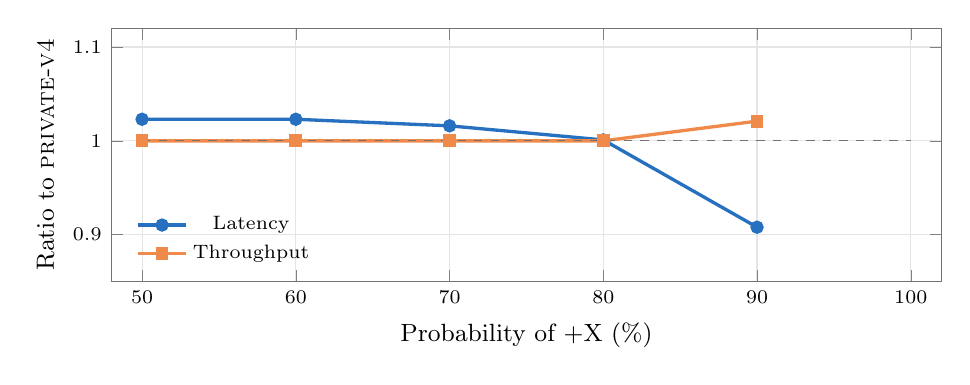
\begin{tikzpicture}
\begin{axis}[
  width=\columnwidth,
  height=4.8cm,
  xmin=48,xmax=102,
  ymin=0.85,ymax=1.12,
  xtick={50,60,70,80,90,100},
  ytick={0.90,1.00,1.10},
  xlabel={Probability of +X (\%)},
  ylabel={Ratio to \privatefour},
  tick label style={font=\scriptsize},
  label style={font=\small},
  legend style={font=\scriptsize,draw=none,fill=none,at={(0.02,0.03)},anchor=south west},
  grid=major,
  grid style={draw=black!10},
  axis line style={draw=black!55}
]
\addplot[tidalblue,very thick,mark=*,mark size=1.8pt]
  coordinates {(50,1.023) (60,1.023) (70,1.016) (80,1.001) (90,0.908)};
\addlegendentry{Latency}
\addplot[tidalorange,very thick,mark=square*,mark size=1.7pt]
  coordinates {(50,1.000) (60,1.000) (70,1.000) (80,1.000) (90,1.021)};
\addlegendentry{Throughput}
\addplot[black!55,dashed] coordinates {(50,1.0) (100,1.0)};
\end{axis}
\end{tikzpicture}
\caption{\capthree under X-direction skew at $L=8$, injection 0.10. The
fully skewed saturated point is excluded from the latency curve.}
\label{fig:skew}
\end{figure}

At 50/50 and 60/40, \system pays a 2.3\% latency penalty because little
cold-side capacity is stranded. The penalty falls to 1.6\% at 70/30 and
approximately breaks even at 80/20. At 90/10, latency falls by 9.2\% while
throughput rises by 2.1\%. At 100\% +X, the private baseline saturates, so a
latency ratio is not a valid below-saturation comparison; the meaningful
observation is 1.818 times delivered throughput during the measurement window.

\begin{figure*}[t]
\centering
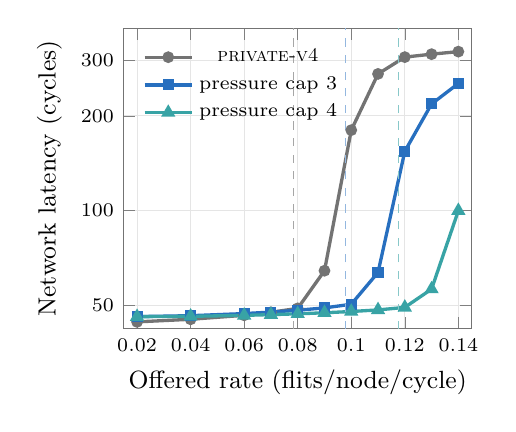
\begin{tikzpicture}
\begin{axis}[
  width=0.495\textwidth, height=5.4cm,
  xmin=0.015, xmax=0.145,
  ymode=log, ymin=42, ymax=380,
  ytick={50,100,200,300}, yticklabels={50,100,200,300},
  xtick={0.02,0.04,0.06,0.08,0.10,0.12,0.14},
  xticklabel style={/pgf/number format/fixed,
    /pgf/number format/precision=2},
  xlabel={Offered rate (flits/node/cycle)},
  ylabel={Network latency (cycles)},
  tick label style={font=\scriptsize},
  label style={font=\small},
  legend style={font=\scriptsize,draw=none,fill=none,
    at={(0.03,0.97)},anchor=north west},
  grid=major, grid style={draw=black!10},
  axis line style={draw=black!55}
]
\addplot[black!55,very thick,mark=*,mark size=1.5pt] coordinates
  {(0.02,44.21) (0.04,45.06) (0.06,46.39) (0.07,47.41) (0.08,48.81)
   (0.09,64.31) (0.1,180.1) (0.11,271.9) (0.12,307.5) (0.13,314.2)
   (0.14,320.1)};
\addlegendentry{\privatefour}
\addplot[tidalblue,very thick,mark=square*,mark size=1.4pt] coordinates
  {(0.02,45.95) (0.04,46.26) (0.06,46.98) (0.07,47.5) (0.08,48.15)
   (0.09,48.98) (0.1,50.3) (0.11,63.52) (0.12,154.2) (0.13,218.2)
   (0.14,253.5)};
\addlegendentry{pressure cap 3}
\addplot[tidalcyan,very thick,mark=triangle*,mark size=1.8pt] coordinates
  {(0.02,45.93) (0.04,46.05) (0.06,46.37) (0.07,46.62) (0.08,46.9)
   (0.09,47.26) (0.1,47.7) (0.11,48.26) (0.12,49.16) (0.13,56.22)
   (0.14,99.82)};
\addlegendentry{pressure cap 4}
\draw[dashed,black!35] (axis cs:0.0784,42) -- (axis cs:0.0784,380);
\draw[dashed,tidalblue!50] (axis cs:0.098,42) -- (axis cs:0.098,380);
\draw[dashed,tidalcyan!60] (axis cs:0.1176,42) -- (axis cs:0.1176,380);
\end{axis}
\end{tikzpicture}\hfill
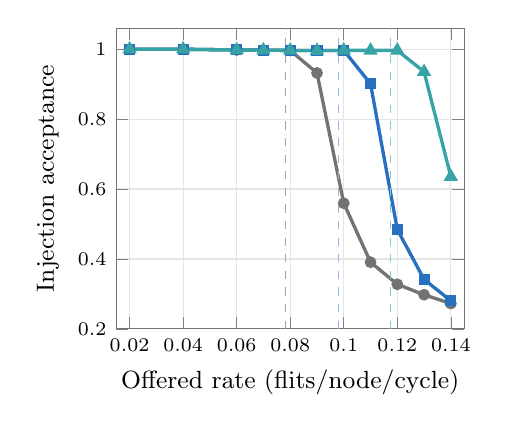
\begin{tikzpicture}
\begin{axis}[
  width=0.495\textwidth, height=5.4cm,
  xmin=0.015, xmax=0.145,
  ymin=0.2, ymax=1.06,
  ytick={0.2,0.4,0.6,0.8,1.0},
  xtick={0.02,0.04,0.06,0.08,0.10,0.12,0.14},
  xticklabel style={/pgf/number format/fixed,
    /pgf/number format/precision=2},
  xlabel={Offered rate (flits/node/cycle)},
  ylabel={Injection acceptance},
  tick label style={font=\scriptsize},
  label style={font=\small},
  grid=major, grid style={draw=black!10},
  axis line style={draw=black!55}
]
\addplot[black!55,very thick,mark=*,mark size=1.5pt] coordinates
  {(0.02,1.0) (0.04,0.9998) (0.06,0.9979) (0.07,0.9971) (0.08,0.9965)
   (0.09,0.9321) (0.1,0.5594) (0.11,0.3908) (0.12,0.3275) (0.13,0.2976)
   (0.14,0.2726)};
\addplot[tidalblue,very thick,mark=square*,mark size=1.4pt] coordinates
  {(0.02,1.0) (0.04,0.9998) (0.06,0.9979) (0.07,0.9971) (0.08,0.9965)
   (0.09,0.996) (0.1,0.9967) (0.11,0.9008) (0.12,0.4842) (0.13,0.3415)
   (0.14,0.2803)};
\addplot[tidalcyan,very thick,mark=triangle*,mark size=1.8pt] coordinates
  {(0.02,1.0) (0.04,0.9998) (0.06,0.9979) (0.07,0.9971) (0.08,0.9965)
   (0.09,0.996) (0.1,0.9967) (0.11,0.9967) (0.12,0.9967) (0.13,0.9353)
   (0.14,0.6353)};
\draw[dashed,black!35] (axis cs:0.0784,0.2) -- (axis cs:0.0784,1.06);
\draw[dashed,tidalblue!50] (axis cs:0.098,0.2) -- (axis cs:0.098,1.06);
\draw[dashed,tidalcyan!60] (axis cs:0.1176,0.2) -- (axis cs:0.1176,1.06);
\end{axis}
\end{tikzpicture}
\caption{Saturation behavior under 100\,\% $+X$ skew at $L=8$
(three-seed means). Dashed rules mark the input-credit bounds
$C/(h\,T_{\mathrm{loop}})=0.078$, $0.098$, $0.118$ for the $C=4$, $5$, $6$
slots each arm's hot input may hold ($h{=}3$ X~hops,
$T_{\mathrm{loop}}{=}17$ cycles). Every measured knee lands on its bound.}
\label{fig:satcurve}
\end{figure*}

Figure~\ref{fig:satcurve} traces the full saturation curves at 100\% skew
with 0.01-step resolution around each knee. Every arm rides flat near 47
cycles until its input credits run out, then collapses within one step:
acceptance breaks between 0.08 and 0.09 for \privatefour, between 0.10 and
0.11 for cap three, and between 0.12 and 0.13 for cap four. Each knee sits
within 2\% of the idealized input-credit bound $C/(h\,T_{\mathrm{loop}})$
implied by Section~\ref{sec:background}---0.078, 0.098, and 0.118 for the
$C=4$, $5$, $6$ slots the arm's hot input may hold. Credit count, not
switch or link bandwidth, is the binding resource here, and moving one or
two idle peer credits raises the stable rate by exactly their share:
25\% for cap three, 50\% for cap four.

\begin{table*}[t]
\centering
\caption{Detailed X-bias sweep at $L=8$, offered rate 0.10. Values are
mean $\pm$ approximate 95\% confidence interval across three seeds; ratios
are computed per seed before averaging. The dagger marks an above-saturation
latency comparison.}
\label{tab:xbias-detail}
\scriptsize
\begin{tabular}{rrrrrrrr}
\toprule
\(+X\) &
\multicolumn{1}{c}{Private thr.} &
\multicolumn{1}{c}{Cap3 thr.} &
\multicolumn{1}{c}{Thr./base} &
\multicolumn{1}{c}{Private net lat.} &
\multicolumn{1}{c}{Cap3 net lat.} &
\multicolumn{1}{c}{Cap3 lat./base} &
\multicolumn{1}{c}{Cap4 lat./base}\\
\midrule
50\%  & .0496$\pm$.0004 & .0496$\pm$.0004 & 1.000$\pm$.000 & 45.86$\pm$.02 & 46.94$\pm$.02 & 1.023$\pm$.000 & 1.018$\pm$.000\\
60\%  & .0496$\pm$.0004 & .0496$\pm$.0004 & 1.000$\pm$.000 & 46.05$\pm$.06 & 47.09$\pm$.04 & 1.023$\pm$.001 & 1.015$\pm$.001\\
70\%  & .0496$\pm$.0004 & .0496$\pm$.0004 & 1.000$\pm$.000 & 46.65$\pm$.08 & 47.39$\pm$.02 & 1.016$\pm$.002 & 1.005$\pm$.002\\
80\%  & .0496$\pm$.0004 & .0496$\pm$.0004 & 1.000$\pm$.000 & 47.91$\pm$.15 & 47.93$\pm$.07 & 1.001$\pm$.002 & .982$\pm$.002\\
90\%  & .0486$\pm$.0013 & .0496$\pm$.0004 & 1.021$\pm$.028 & 53.94$\pm$4.68 & 48.78$\pm$.07 & .908$\pm$.075 & .880$\pm$.074\\
100\% & .0273$\pm$.0008 & .0496$\pm$.0004 & 1.818$\pm$.061 & 180.14$\pm$8.17 & 50.30$\pm$.24 & .280$\pm$.012$^\dagger$ & .265$\pm$.012$^\dagger$\\
\bottomrule
\end{tabular}
\end{table*}

\begin{figure}[t]
\centering
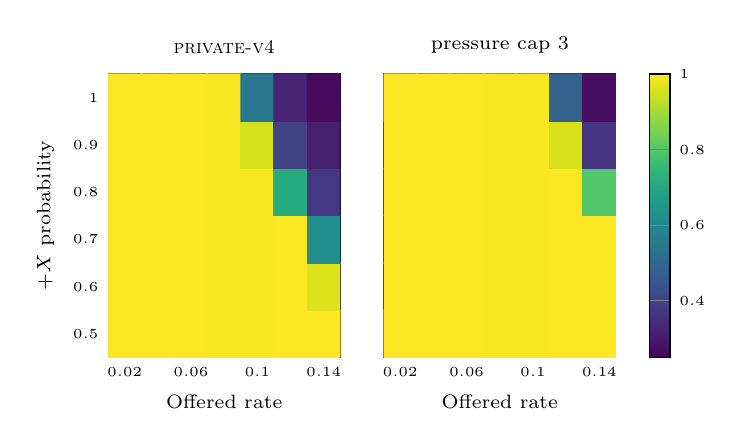
\begin{tikzpicture}
\begin{axis}[
  name=hma,
  width=2.95cm, height=3.6cm, scale only axis,
  view={0}{90}, colormap/viridis,
  point meta min=0.25, point meta max=1.0,
  xmin=0.01, xmax=0.15, ymin=0.45, ymax=1.05,
  xtick={0.02,0.06,0.10,0.14}, ytick={0.5,0.6,0.7,0.8,0.9,1.0},
  xticklabel style={/pgf/number format/fixed,
    /pgf/number format/precision=2},
  tick label style={font=\tiny},
  label style={font=\scriptsize},
  xlabel={Offered rate}, ylabel={$+X$ probability},
  title={\privatefour}, title style={font=\scriptsize,yshift=-2pt}
]
\addplot[matrix plot*, point meta=explicit, mesh/cols=7]
table[x index=0, y index=1, meta index=2, header=false] {
0.02 0.5 0.999
0.04 0.5 1.000
0.06 0.5 0.999
0.08 0.5 0.996
0.10 0.5 0.996
0.12 0.5 0.997
0.14 0.5 0.997
0.02 0.6 0.999
0.04 0.6 1.000
0.06 0.6 0.999
0.08 0.6 0.996
0.10 0.6 0.996
0.12 0.6 0.997
0.14 0.6 0.963
0.02 0.7 0.999
0.04 0.7 1.000
0.06 0.7 0.999
0.08 0.7 0.996
0.10 0.7 0.996
0.12 0.7 0.997
0.14 0.7 0.617
0.02 0.8 0.999
0.04 0.8 1.000
0.06 0.8 0.999
0.08 0.8 0.996
0.10 0.8 0.996
0.12 0.8 0.711
0.14 0.8 0.372
0.02 0.9 0.999
0.04 0.9 1.000
0.06 0.9 0.999
0.08 0.9 0.996
0.10 0.9 0.952
0.12 0.9 0.401
0.14 0.9 0.310
0.02 1.0 0.999
0.04 1.0 1.000
0.06 1.0 0.999
0.08 1.0 0.996
0.10 1.0 0.550
0.12 1.0 0.327
0.14 1.0 0.273
};
\end{axis}
\begin{axis}[
  at={(hma.south east)}, anchor=south west, xshift=0.55cm,
  width=2.95cm, height=3.6cm, scale only axis,
  view={0}{90}, colormap/viridis,
  point meta min=0.25, point meta max=1.0,
  xmin=0.01, xmax=0.15, ymin=0.45, ymax=1.05,
  xtick={0.02,0.06,0.10,0.14}, ytick={0.5,0.6,0.7,0.8,0.9,1.0},
  yticklabels={},
  xticklabel style={/pgf/number format/fixed,
    /pgf/number format/precision=2},
  tick label style={font=\tiny},
  label style={font=\scriptsize},
  xlabel={Offered rate},
  title={pressure cap 3}, title style={font=\scriptsize,yshift=-2pt},
  colorbar,
  colorbar style={width=2.6mm, tick label style={font=\tiny}}
]
\addplot[matrix plot*, point meta=explicit, mesh/cols=7]
table[x index=0, y index=1, meta index=2, header=false] {
0.02 0.5 0.999
0.04 0.5 1.000
0.06 0.5 0.999
0.08 0.5 0.996
0.10 0.5 0.996
0.12 0.5 0.997
0.14 0.5 0.997
0.02 0.6 0.999
0.04 0.6 1.000
0.06 0.6 0.999
0.08 0.6 0.996
0.10 0.6 0.996
0.12 0.6 0.997
0.14 0.6 0.997
0.02 0.7 0.999
0.04 0.7 1.000
0.06 0.7 0.999
0.08 0.7 0.996
0.10 0.7 0.996
0.12 0.7 0.997
0.14 0.7 0.997
0.02 0.8 0.999
0.04 0.8 1.000
0.06 0.8 0.999
0.08 0.8 0.996
0.10 0.8 0.996
0.12 0.8 0.997
0.14 0.8 0.799
0.02 0.9 0.999
0.04 0.9 1.000
0.06 0.9 0.999
0.08 0.9 0.996
0.10 0.9 0.996
0.12 0.9 0.955
0.14 0.9 0.365
0.02 1.0 0.999
0.04 1.0 1.000
0.06 1.0 0.999
0.08 1.0 0.996
0.10 1.0 0.996
0.12 1.0 0.483
0.14 1.0 0.279
};
\end{axis}
\end{tikzpicture}
\caption{Injection acceptance over the bias--rate grid at $L=8$
(single seed). Bright cells accept the offered load; dark cells are
saturated. Cap three loses no cell, matches the baseline at balanced
bias, and pushes the stable frontier one 0.02 step right wherever the
skew probability is at least 0.7.}
\label{fig:biasmap}
\end{figure}

Figure~\ref{fig:biasmap} maps the operating region over the full
bias--rate grid. Cap three's stable region strictly contains the
baseline's: no cell is worse, the two maps coincide at balanced 50\%
bias, and for bias probabilities of 0.7 and above the acceptance
frontier sits one 0.02 grid step further right---17--25\% more stable
offered rate precisely where skew persists. The map also bounds the
mechanism's reach: below the private credit bound every organization is
equivalent, so \system's case rests entirely on the band between the
private and pooled frontiers.

\subsection{Tornado and policy comparison}

On 4$\times$4$\times$4, torus tornado advances each packet by +1 in X, +1 in
Y, and +1 in Z, making W, S, and D true inputs persistently hot.
Figure~\ref{fig:tornado-curve} sweeps the offered rate at $L=8$;
Table~\ref{tab:tornado} details the saturated 0.9 point.

\begin{figure*}[t]
\centering
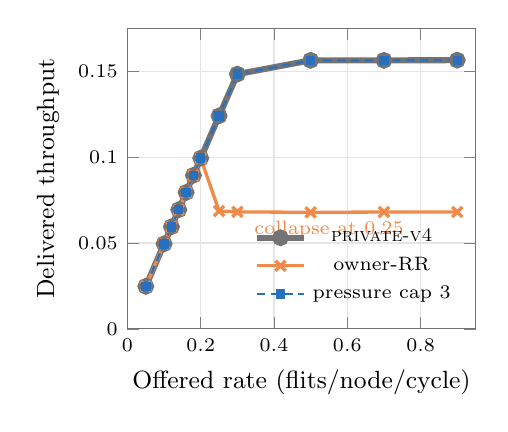
\begin{tikzpicture}
\begin{axis}[
  width=0.495\textwidth, height=5.4cm,
  xmin=0, xmax=0.95,
  ymin=0, ymax=0.175,
  ytick={0,0.05,0.10,0.15},
  yticklabel style={/pgf/number format/fixed,
    /pgf/number format/precision=2},
  xtick={0,0.2,0.4,0.6,0.8},
  xlabel={Offered rate (flits/node/cycle)},
  ylabel={Delivered throughput},
  tick label style={font=\scriptsize},
  label style={font=\small},
  legend style={font=\scriptsize,draw=none,fill=none,
    at={(0.97,0.05)},anchor=south east},
  grid=major, grid style={draw=black!10},
  axis line style={draw=black!55}
]
\addplot[black!55,line width=2.2pt,mark=*,mark size=1.9pt] coordinates
  {(0.05,0.02476) (0.1,0.04952) (0.12,0.05943) (0.14,0.06936)
   (0.16,0.07942) (0.18,0.08941) (0.2,0.0994) (0.25,0.124) (0.3,0.1483)
   (0.5,0.1563) (0.7,0.1563) (0.9,0.1564)};
\addlegendentry{\privatefour}
\addplot[tidalorange,very thick,mark=x,mark size=2.6pt] coordinates
  {(0.05,0.02476) (0.1,0.04951) (0.12,0.05941) (0.14,0.06933)
   (0.16,0.07938) (0.18,0.08933) (0.2,0.09927) (0.25,0.06861)
   (0.3,0.0681) (0.5,0.06784) (0.7,0.06802) (0.9,0.06804)};
\addlegendentry{owner-RR}
\addplot[tidalblue,thick,densely dashed,mark=square*,mark size=1.3pt,
  mark options={solid}] coordinates
  {(0.05,0.02476) (0.1,0.04951) (0.12,0.05942) (0.14,0.06935)
   (0.16,0.07941) (0.18,0.0894) (0.2,0.09939) (0.25,0.124) (0.3,0.1483)
   (0.5,0.1562) (0.7,0.1563) (0.9,0.1563)};
\addlegendentry{pressure cap 3}
\node[font=\scriptsize,text=tidalorange,anchor=west]
  at (axis cs:0.32,0.058) {collapse at 0.25};
\end{axis}
\end{tikzpicture}\hfill
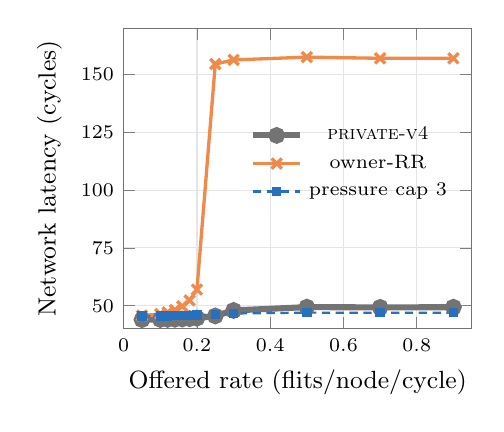
\begin{tikzpicture}
\begin{axis}[
  width=0.495\textwidth, height=5.4cm,
  xmin=0, xmax=0.95,
  ymin=40, ymax=170,
  ytick={50,75,100,125,150},
  xtick={0,0.2,0.4,0.6,0.8},
  xlabel={Offered rate (flits/node/cycle)},
  ylabel={Network latency (cycles)},
  tick label style={font=\scriptsize},
  label style={font=\small},
  legend style={font=\scriptsize,draw=none,fill=none,
    at={(0.97,0.55)},anchor=east},
  grid=major, grid style={draw=black!10},
  axis line style={draw=black!55}
]
\addplot[black!55,line width=2.2pt,mark=*,mark size=1.9pt] coordinates
  {(0.05,44.02) (0.1,44.07) (0.12,44.12) (0.14,44.18) (0.16,44.27)
   (0.18,44.42) (0.2,44.64) (0.25,45.59) (0.3,47.98) (0.5,49.41)
   (0.7,49.3) (0.9,49.37)};
\addlegendentry{\privatefour}
\addplot[tidalorange,very thick,mark=x,mark size=2.6pt] coordinates
  {(0.05,45.75) (0.1,46.43) (0.12,47.1) (0.14,48.16) (0.16,49.77)
   (0.18,52.33) (0.2,56.99) (0.25,154.5) (0.3,156.3) (0.5,157.5)
   (0.7,157) (0.9,157)};
\addlegendentry{owner-RR}
\addplot[tidalblue,thick,densely dashed,mark=square*,mark size=1.3pt,
  mark options={solid}] coordinates
  {(0.05,45.65) (0.1,45.59) (0.12,45.63) (0.14,45.68) (0.16,45.77)
   (0.18,45.86) (0.2,45.96) (0.25,46.24) (0.3,46.65) (0.5,47.03)
   (0.7,47) (0.9,46.97)};
\addlegendentry{pressure cap 3}
\end{axis}
\end{tikzpicture}
\caption{Tornado sweep at $L=8$ (three-seed means; cap 4 overlays cap 3
and is omitted). Left: pressure tracks the private baseline to saturation,
while blind owner rotation collapses at rate 0.25 and never recovers.
Right: below saturation the phase schedule costs pressure a flat
1.6~cycles; past the output knee near 0.3 the order reverses and pressure
finishes 2.4~cycles below the baseline.}
\label{fig:tornado-curve}
\end{figure*}

\begin{table*}[t]
\centering
\caption{Tornado policy comparison at offered rate 0.9. Values are
mean $\pm$ approximate 95\% confidence interval over three seeds. Pool,
reclaim, and handoff columns are percentages of completed control events.}
\label{tab:tornado}
\scriptsize
\begin{tabular}{rrlrrrrrr}
\toprule
L & Mode & Throughput & Thr./base & Net latency & Lat./base &
Pool service & Reclaim & Handoff\\
\midrule
1 & \privatefour & .4489$\pm$.0003 & 1.000 & 10.46$\pm$.00 & 1.000 & -- & -- & --\\
1 & Owner-RR & .3138$\pm$.0013 & .699$\pm$.003 & 32.08$\pm$.16 & 3.067$\pm$.016 & 25.37 & .00 & .11\\
1 & Pressure cap3 & .4488$\pm$.0003 & 1.000$\pm$.000 & 13.09$\pm$.01 & 1.251$\pm$.001 & 59.11 & .13 & .09\\
\midrule
8 & \privatefour & .1564$\pm$.0000 & 1.000 & 49.37$\pm$.07 & 1.000 & -- & -- & --\\
8 & Owner-RR & .0680$\pm$.0004 & .435$\pm$.003 & 157.03$\pm$1.16 & 3.181$\pm$.022 & 27.67 & .00 & .44\\
8 & Pressure cap3 & .1563$\pm$.0000 & 1.000$\pm$.000 & 46.97$\pm$.03 & .952$\pm$.002 & 66.38 & .49 & .40\\
\bottomrule
\end{tabular}
\end{table*}

Pressure cap three lowers latency by 4.85\% without changing throughput
materially because an output bottleneck limits tornado first. It captures
about 83\% of the latency benefit of cap four while preserving one peer
credit. Only approximately 0.49\% of \pool allocations use on-demand reclaim:
stable ownership handles most demand, and reclaim resolves occasional
mismatches. Owner round-robin loses 56.5\% throughput because blind rotation
can place credits at an inactive peer and has no demand-driven correction.

The rate sweep separates the failure modes. Below the output-bandwidth
knee near 0.3, all demand-aware arms deliver identical throughput and the
phase schedule costs the \system arms a flat 1.6 cycles of latency over
\privatefour; past the knee the order reverses and pressure rides 2.4
cycles below the baseline. Owner-RR is qualitatively different: its
latency climbs from rate 0.1 onward, and at 0.25 its delivered throughput
collapses to 0.068 and never recovers---misplaced credits, not bandwidth,
are its binding resource.

\begin{table}[t]
\centering
\caption{Owner-cap ablation for tornado, $L=8$, rate 0.9.}
\label{tab:cap}
\small
\setlength{\tabcolsep}{4pt}
\begin{tabular}{lrrrr}
\toprule
Mode & Lat. & Lat./base & Reclaim & Borrow peak\\
\midrule
\privatefour & 49.37 & 1.000 & -- & 0\\
Cap 2 & 58.25 & 1.180 & 0.00\% & 0\\
Cap 3 & 46.97 & .952 & .49\% & 1\\
Cap 4 & 46.47 & .941 & .19\% & 2\\
\bottomrule
\end{tabular}
\end{table}

Cap two prevents borrowing and is behaviorally equivalent to static
ownership. Cap three recovers most of cap four's latency benefit while
retaining one credit at the cold side. Cap four is slightly faster here but
can temporarily leave the peer with no Pool ownership.

\begin{table}[t]
\centering
\caption{Credit/control event counts for pressure cap 3 under tornado,
$L=8$, rate 0.9. Counts are rounded three-seed means per 10,000-cycle run.}
\label{tab:events}
\scriptsize
\begin{tabular}{lr@{\qquad}lr}
\toprule
Counter & Mean & Counter & Mean\\
\midrule
Pool allocations & 202,267 & Owned allocations & 201,267\\
Demand reclaims & 1,000 & Owner migrations & 1,809\\
Release handoffs & 809 & Release keeps & 201,274\\
Pool reads & 202,083 & RES reads & 102,347\\
Pool write blocks & 0 & Pool read conflicts & 0\\
Borrowed peak & 1 & Deadlocks & 0\\
\bottomrule
\end{tabular}
\end{table}

The event identities are visible numerically:
\(202{,}267=201{,}267+1{,}000\) allocations and
\(1{,}809=1{,}000+809\) migrations. Completed Pool reads also equal released
keeps plus handoffs, \(202{,}083=201{,}274+809\); the allocation/read
difference is the set of flits still resident at measurement end. Zero
write-block counts mean the allocator never committed a second Pool write in
the same pair-cycle in these runs; this validates the guard's behavior, not
the timing or area of a fabricated 1W array.

\subsection{Where 1R1W loses}

The phase schedule is a real bandwidth constraint. Against \privatefour,
uniform traffic at $L=8$, injection 0.9 raises latency by approximately 3.2\%.
X-opposite traffic raises latency by 3--15\% because both members of a pair
compete for one shared read. Tornado at $L=1$ raises latency by 25.1\% because
the credit loop is too short for additional capacity to repay the phase cost.
Reversing the hot X direction every 16 cycles raises latency by 7.8\% while
ownership and old traffic drain in opposite directions.

\begin{table}[t]
\centering
\caption{Representative pressure-cap3 losses. Ratios are against equal-storage
\privatefour. The X-opposite row is a 3,000-cycle single-seed smoke point; the
others are 10,000-cycle, three-seed results.}
\label{tab:negative}
\scriptsize
\begin{tabular}{llrr}
\toprule
Traffic / condition & $L$ & Thr./base & Lat./base\\
\midrule
Uniform, rate .9 & 8 & 1.001 & 1.032\\
X-opposite, rate .9 & 8 & .999 & 1.154\\
Tornado, rate .9 & 1 & 1.000 & 1.251\\
X reversal, epoch 16 & 8 & .999 & 1.078\\
\bottomrule
\end{tabular}
\end{table}

\begin{table}[t]
\centering
\caption{Direction-reversal sensitivity at $L=8$, rate 0.9. Counts and
absolute values are three-seed means.}
\label{tab:reversal}
\scriptsize
\setlength{\tabcolsep}{3.4pt}
\begin{tabular}{rrrrrr}
\toprule
Epoch & Base thr. & Cap3 thr. & Base lat. & Cap3 lat. & Migrations\\
\midrule
4   & .1575 & .1575 & 27.37 & 27.97 & 5,335\\
16  & .1560 & .1559 & 28.49 & 30.72 & 16,707\\
64  & .1549 & .1558 & 27.77 & 28.60 & 7,649\\
256 & .1565 & .1567 & 26.63 & 27.26 & 2,428\\
\bottomrule
\end{tabular}
\end{table}

The epoch-16 point is worst because ownership moves most often while the
previous direction's flits are still draining. Very fast four-cycle reversal
leaves little time to build an extreme ownership split; long epochs amortize
each transition. This is direct evidence that credit policy must be evaluated
as a dynamic controller, not only by its steady-state cap.

VC scaling supports the same interpretation. Near the measured knee, a
six-VC organization reaches a 1.27 throughput ratio and a 0.56 latency ratio,
extending the stable bracket from 0.12 to 0.15. At eight VCs, where private
capacity already hides more of the credit loop, the ratios shrink to 1.08 and
0.83, extending 0.18 to 0.20.

\subsection{Data provenance}

The raw rows used above are tracked under
\path{1R1W/overlay/lab/DP/physical_bound/}. Table~\ref{tab:matrix} names each
CSV exactly; the revision's curve and map rows live in
\path{results_xbias_curve.csv}, \path{results_tornado_curve.csv}, and
\path{results_bias_heatmap.csv}. \path{run_sweep_dpphys.py} records the gem5
command for every run, and \path{analyze_dpphys.py} performs paired-by-seed
ratios and confidence-interval aggregation. The archived overlay should be reconstructed
in a temporary worktree from base commit \path{2eb6a4e}; it should not be
copied over the repository's current working source.

\section{Hardware Interpretation}

The evaluated comparison establishes equal buffer capacity and a one-read,
one-write \pool service limit. This is a plausible manufacturing advantage
over an ideal shared bank that must serve both directions simultaneously, but
it is not yet an area or energy result. \system adds the control state,
selectors, arbiters, and ownership sideband of Section~\ref{sec:physical};
the state itself is under 5\% of the pair's data bits, but the selectors and
the ownership update path can be timing-critical. We therefore claim reduced
shared-port demand, not zero hardware cost. RTL synthesis against private and dual-access pool
implementations is required to quantify area, energy, and frequency.

This comparison explains both the intended cost saving and the performance
losses. Relative to an unrestricted 2R2W shared pool, \system removes one
shared read and one shared write service, reducing the hardest shared-port
requirement. Relative to private banks, however, it adds a central selection
and ownership path. Whether the smaller Pool port count outweighs those
selectors depends on entry width, SRAM/register-file implementation, wire
length, and target frequency. Garnet cannot answer that manufacturing
question. The ordinary router allocator and crossbar remain present in all
three organizations~\cite{dallytowles2004}.

\section{Limitations and Next Steps}
\label{sec:limits}

The present evidence is preliminary and simulator-level. First, demand reclaim
updates ownership with zero additional cycles; a one-cycle and parameterized
grant path should measure timing sensitivity. Second, finer 0.005 injection
steps, longer drain-aware runs, and at least five seeds are needed around every
saturation knee. Third, a directed simultaneous E/W-write microbenchmark
should stress the write guard. Fourth, multi-flit packets require an explicit
packet/VC ownership-retention rule. Finally, RTL synthesis should compare
private buffers, 1R1W \system, and an idealized dual-access pool.

\section{Related Work}

Virtual-channel flow control and its buffer/throughput tradeoffs were
formalized by Dally~\cite{dally1992virtual}. Deadlock-free routing can be
constructed through channel-dependency restrictions~\cite{dally1987deadlock}
or broader adaptive conditions~\cite{duato1993theory}; \system preserves a
private deterministic escape resource rather than changing those guarantees.
Garnet provides the detailed router and credit model used
here~\cite{agarwal2009garnet}, inside the gem5 simulation
infrastructure~\cite{binkert2011gem5}. Shared-buffer organizations and
industrial credit pools are positioned in Section~\ref{sec:background};
relative to both lines, our contribution is the combination of
direction-paired equal-capacity storage spanning two opposing inports, a
structurally 1R1W shared bank, and demand-aware ownership credits.

\section{Division of Labor}

The project was completed with equal overall contribution: Changxun Pan 50\%
and Liming Wang 50\%. Both contributors participated in architecture
discussion, debugging, correctness review, experiment review, interpretation,
writing, slide production, and presentation preparation.

\textbf{Liming Wang} proposed the original direction-paired pooling concept,
implemented and evaluated an earlier 1R2W prototype, expanded traffic and
evaluation coverage, reviewed and improved the 1R1W and credit-policy behavior, and
co-analyzed and co-authored the final deliverables.

\textbf{Changxun Pan} co-developed the design and finalized its complementary
1R1W phase schedule, designed pressure, sticky-tie, cap-three, and reclaim control,
implemented the final mechanism and instrumentation, ran and cross-checked
major 1R1W experiments, and co-analyzed and co-authored the final deliverables.

\section{Conclusion}

\system shows that buffer elasticity does not require an unconstrained global
pool. Pairing opposite directions and preserving private escape capacity lets
a four-slot adaptive pool move storage toward sustained pressure while
retaining equal total capacity. A complementary schedule enforces one shared
read and one shared write per cycle. The design is effective under persistent
directional skew and long credit loops, but balanced demand, short links, and
fast reversals expose its serialized-access cost. Pressure-aware credit
movement is essential: blind ownership rotation is substantially worse. The
next decisive step is to add grant delay and synthesize the control and
storage organization so that performance gains can be judged against measured
area, energy, and timing.

{\small
\bibliographystyle{abbrv}
\bibliography{tidal_1r1w_refs}
}

\end{document}
